\chapter{Introduction}

\endquote{``\emph{All problems in computer science can be solved by another
    level of indirection.}''

  \hfill\footnotesize --- David Wheeler}

\vspace{1cm}\noindent To manage complexity, computing platforms are commonly
built as successions of abstraction layers, from the hardware architecture's
components up to high-level software applications.
%
Each layer leverages the interface of its predecessor to expose a higher-level,
more constrained set of functionalities for its successors.
%
This enables separation of concerns ---each layer encapsulates one dimension of
the overall complexity--- and modularity ---two layers which expose the same
interface can be seamlessly interchange---.

A layer is often \emph{more privileged} than, and therefore implicitly trusted
by, its successors.
%
From a security perspective, the former may constrain the latter, with respect
to targeted security properties.
%
For instance, an operating system shares hardware resources among several
applications, and therefore is able to enforce availability ---fair share of CPU
time---, confidentiality and integrity ---exclusive partition of physical
memories--- properties.
%
Constraining one's execution can be achieved in various ways.
%
Concerning the lowest layers of a software stack, the common approach is to rely
on features provided by the hardware architecture.
%
For instance, mainstream operating systems leverage, among others mechanisms, a
\emph{Memory Management Unit} (MMU) to partition the system memory and a
hardware timer to schedule arbitrary applications.

\section{Hardware-based Security Enforcement mechanisms}

We call this class of security enforcement mechanisms, where a trusted software
component configure the underlying hardware architecture to constrain the
execution of untrusted and potentially arbitrary software components,
\emph{Hardware-based Security Enforcement} (HSE).

A HSE mechanism is correct, \emph{i.e.} it enforces the targeted security
property, when both the hardware features are correctly implemented and the
software components correctly configure them.
%
Both remain challenging.
%
Over the past decades, vendors have added many security features to their
products.
%
Intel, for instance, have notably introduced hardware-based virtualization
(VT-x, VT-d), dynamic root of trust (TXT), or applicative enclaves (SGX).
%
Most of them have been compromised at least once.
%
At the same time, it has been repeatedly shown that vendors were not always
correctly taking advantage of important hardware features at their disposal.
%
These lacks of hardware configuration put the affected computing platforms at
risk.
%
Many security vulnerabilities disclosed over the years have been the result of a
misconfiguration of hardware features by key software components.

In addition, hardware architecture often comprise hundreds of features
implemented by dozens of interconnected devices.
%
This paves the road for a class of security vulnerabilities we call
\emph{architectural attacks}, where each component is working as expected, yet
their composition creates an attack path.
%
This latter class of security vulnerabilities differs from the two other,
because it concerns the specifications of the computing platform rather than its
implementations.

\section{Towards Formal Verification}

In this thesis, our initial objective is to formally specify HSE mechanisms,
which implies defining both the targeted security property and the required
configuration steps trusted software components have to performed.
%
Such unambiguous, security-focused specification can be leverage by software
developers, as a complement to the existing hardware specifications.
%
Furthermore, this initial specification effort aims to serve as a premise for
verifying the underlying hardware architecture.
%
More precisely, we want to verify if, at least at a specification level, the
hardware architecture effectively enforce the expected security property.
%
Commodity hardware architectures pose several challenge regarding
this task.

%   \begin{figure}
%     \centering
%  %     \includestandalone[width=.8\textwidth]{Figures/intro-computing-platform}
%     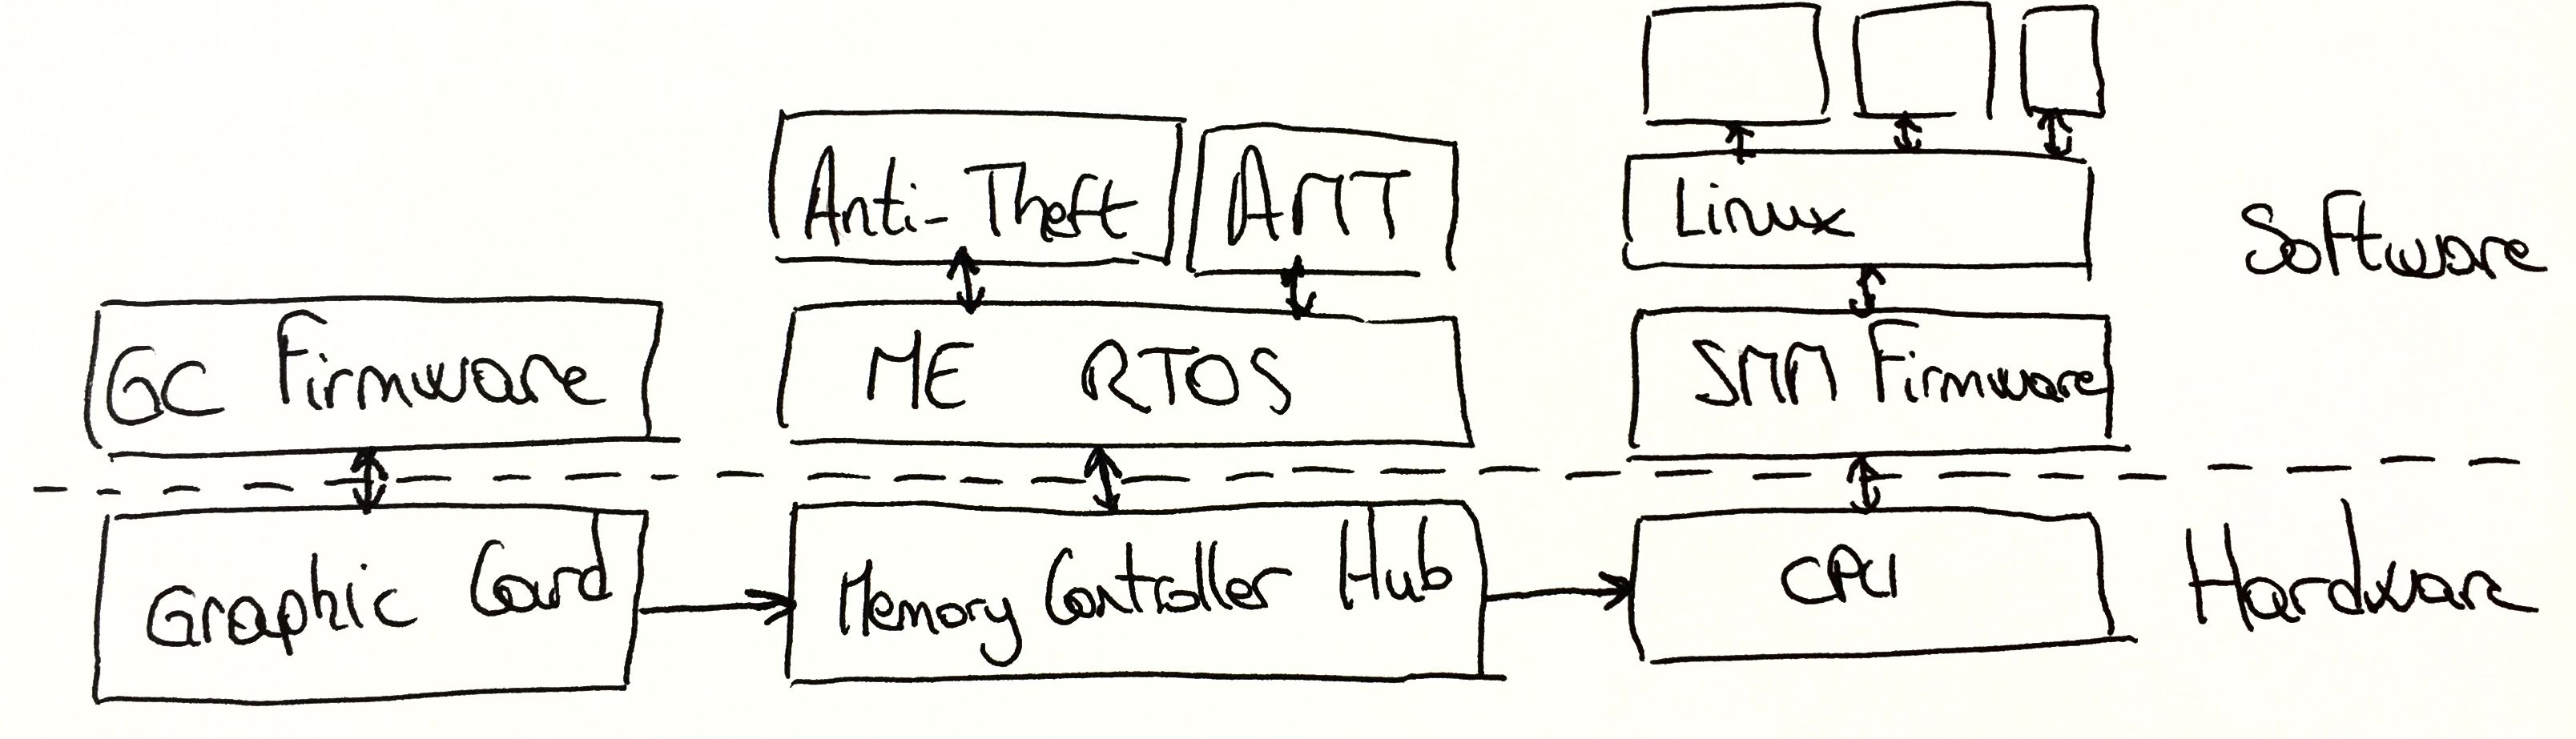
\includegraphics[width=0.8\textwidth]{Figures/intro-computing-platform.jpg}
%     \caption{Abstraction Layers of a Typical x86 Computing Platform}
%     \label{fig:intro:computing-platform}
%   \end{figure}

%   This makes \emph{isolation} a key security property.
% %
%   In the context of this thesis, we say one component $A$ is said isolated
%   from a second component $B$ when $B$ cannot tamper with $A$'s functioning
%   otherwise than through its interface.
% %
%   Thus, an operating system should be isolated from end users applications, to
%   prevent the latter to grant themselves abusive rights.
% %
%   The opposite is not necessarily true, and it is even a common practice for
%   operating system to tamper with applications code (\emph{e.g.} address space
%   layout randomization, dynamic libraries).

\section{Contributions}
